\documentclass[11pt,a4paper]{article}
\usepackage{fontspec}
\setmainfont{TeX Gyre Pagella}
\newfontfamily\headfont{Inter}[UprightFont=*-ExtraBold,BoldFont=*-ExtraBold,Extension=.otf,Path=/usr/share/fonts/opentype/inter/]
\usepackage[a4paper,margin=2.3cm]{geometry}
\usepackage{graphicx,booktabs,float,caption,array,xcolor,longtable}
\usepackage{xurl}
\usepackage[hidelinks]{hyperref}
\usepackage{titlesec}
\usepackage[round]{natbib}
\usepackage{setspace}
\setstretch{1.05}
\renewcommand{\topfraction}{0.9}
\renewcommand{\bottomfraction}{0.8}
\renewcommand{\textfraction}{0.1}
\renewcommand{\floatpagefraction}{0.75}
\setlength{\parindent}{0pt}
\setlength{\parskip}{0.55em}
\titleformat{\section}{\headfont\Large}{\thesection}{0.8em}{}
\titleformat{\subsection}{\headfont\large}{\thesubsection}{0.8em}{}
\captionsetup{font=small,labelfont=bf}
\urlstyle{same}
\hypersetup{pdftitle={The Middle of Nowhere},pdfauthor={Tristan Hotham}}

\begin{document}
\begin{center}
{\Large\bfseries The Middle of Nowhere\par}
\vspace{0.4em}
{\large The most remote places on Earth, measured from every town:\\distances from all land to 171,737 populated places, cities and the coast\par}
\vspace{1.2em}
{\large Tristan Hotham\par}
\vspace{0.3em}
{\small Independent researcher\\
ORCID: 0000-0003-4931-9349\\
DOI: https://doi.org/10.5281/zenodo.23873015\par}
\vspace{0.8em}
2026
\end{center}

\begin{quote}
\small
\begin{center}\textbf{Abstract}\end{center}
Poles of inaccessibility are usually defined as the points farthest from the sea. I compute a different kind of remoteness: the great-circle distance from every point on land to the nearest populated place of 1,000 or more people in the GeoNames gazetteer (171,737 places), to the nearest city of 100,000 or more and of 1,000,000 or more in Natural Earth, and to the nearest coast, on an area-weighted 0.1 degree grid of 2,147,063 land cells, with maxima refined to 0.01 degrees. Outside Antarctica, 24.6\% of the land (33.1 million km\textsuperscript{2}) is more than 100 km from a town and 1.3\% more than 500 km; half lies within 40 km. Land north of 60\textdegree N holds 35\% of the land beyond 100 km and 93\% of that beyond 500 km. The most remote point on each mainland is Cape Chelyuskin in Asia (641 km), the Great Victoria Desert in Australia (579 km), the Libyan Desert of Sudan in Africa (517 km), northern Saskatchewan in North America (506 km), northern Par\'a in South America (364 km) and north-eastern European Russia (288 km). Counting islands, Marion Island is the most remote land outside Antarctica (1,749 km), and every point in Antarctica, which has no towns in the gazetteer, is at least 879 km from one. The classic far-from-the-sea pole in Dzungaria lies only 65 km from a town. In the United Kingdom the most remote spot is near Cape Wrath (82 km); England's is in Kielder Forest (24 km) and its nearest town is in Scotland. I report the most remote point of every country and territory and discuss the limits of straight-line distance to a gazetteer.

\textbf{Keywords:} remoteness; pole of inaccessibility; settlement; accessibility; GeoNames; Natural Earth; great-circle distance; wilderness; open data; mapping
\end{quote}

\section{Introduction}
The idea of a pole of inaccessibility, the point on a continent or ocean farthest from the coast, has a long history in exploration and cartography, and its best known example, the Eurasian pole in the Dzungarian basin of north-west China, has been computed many times. Distance from the sea, however, says little about isolation from people. A point can be thousands of kilometres from any ocean and an hour's drive from a market town.

This paper computes remoteness from settlement instead. For every point on land I measure the great-circle distance to the nearest populated place of 1,000 or more people, to the nearest city of 100,000 or more and of a million or more, and, for comparison, to the nearest coast. I then report how much of the world's land is far from a town, where the most remote point of each continent, large island and country lies, and what the same measure finds in a densely settled country, the United Kingdom. The results accompany an interactive map (\url{https://maps.tristanhotham.com/remote-places/}).

\section{Data}
\textbf{Towns.} The GeoNames cities1000 file \citep{geonames} lists every populated place with 1,000 or more people, together with some smaller places that are seats of administrative divisions; I use the copy packaged by \citet{citiesjson} (commit e5e759c56751bd7329e29c576f6a9e77607b424e), with 171,737 places in 246 countries and territories. It has names, coordinates and country codes but no populations. None of its places lies south of 60\textdegree S.

\textbf{Cities.} Natural Earth's populated places \citep{naturalearth} give estimated populations (pop\_max) for 7,342 places, of which 3,089 have 100,000 or more people and 505 a million or more.

\textbf{Land, coast and countries.} The Natural Earth 1:50m land polygons define land and coast; lakes count as land and the Caspian Sea as sea, and the Antarctic outline follows the land rather than the floating ice shelves. Countries and territories are the Natural Earth 1:10m admin 0 polygons; the 1:10m first-level divisions split the United Kingdom into its four nations and name council areas.

\section{Method}
\textbf{Grid.} A 0.1 degree latitude and longitude grid (3,600 by 1,800 cells) is laid over the land. A cell is land if its centre falls inside the land polygons; cells along the coast are tested exactly (128,817 cells) and the rest are rasterised, which agrees with an exact test on 99.92\% of a random sample. This gives 2,147,063 land cells. Each cell is weighted by its true area on the sphere, $R^2\,\Delta\lambda\,(\sin\phi_2-\sin\phi_1)$, so that the narrow cells near the poles are not over-counted; total land is 146,987,097 km\textsuperscript{2}, of which Antarctica is 12,269,499 km\textsuperscript{2}.

\textbf{Distances.} Every town, city and coast point (the land outline densified to 0.02 degrees, 458,716 points) is converted to a unit vector, and the nearest one to each cell centre is found with a k-d tree. The chord length $c$ to the nearest point gives the great-circle distance exactly as $2R\arcsin(c/2)$, with $R = 6371.0$ km.

\textbf{Maxima.} For each region (the world, a continent's mainland, an island, a country) the best few grid cells are refined on a 0.01 degree grid within 0.1 degrees of each, keeping only points inside the region's polygon. Positions are therefore good to about a kilometre. A country's most remote point is the point inside its outline farthest from any town, in that country or not; I also report the same for each country's largest polygon, its main land mass.

\textbf{Continents.} Continents follow Natural Earth's country assignment, with Russia split along a rough line for the Urals and the Kara Sea. A mainland is the Natural Earth land polygon of the continent; at 1:50m a few islands separated by very narrow straits are joined to it. Antarctica is reported separately throughout: with no towns in the gazetteer, every Antarctic distance is to a town on another continent, so including it would swamp the world shares.

\section{Results}
\subsection{How much land is far from a town}
Half of the land outside Antarctica lies within 40 km of a town, and 36\% within 25 km (Figure~\ref{fig:share}). 24.6\% is more than 100 km away, 6.7\% more than 250 km and 1.3\% more than 500 km. The medians for cities of 100,000 and of a million are 175 km and 458 km, and 46.4\% of the land is more than 500 km from a city of a million. Half of the land is within 400 km of the coast.

\begin{figure}[tbp]\centering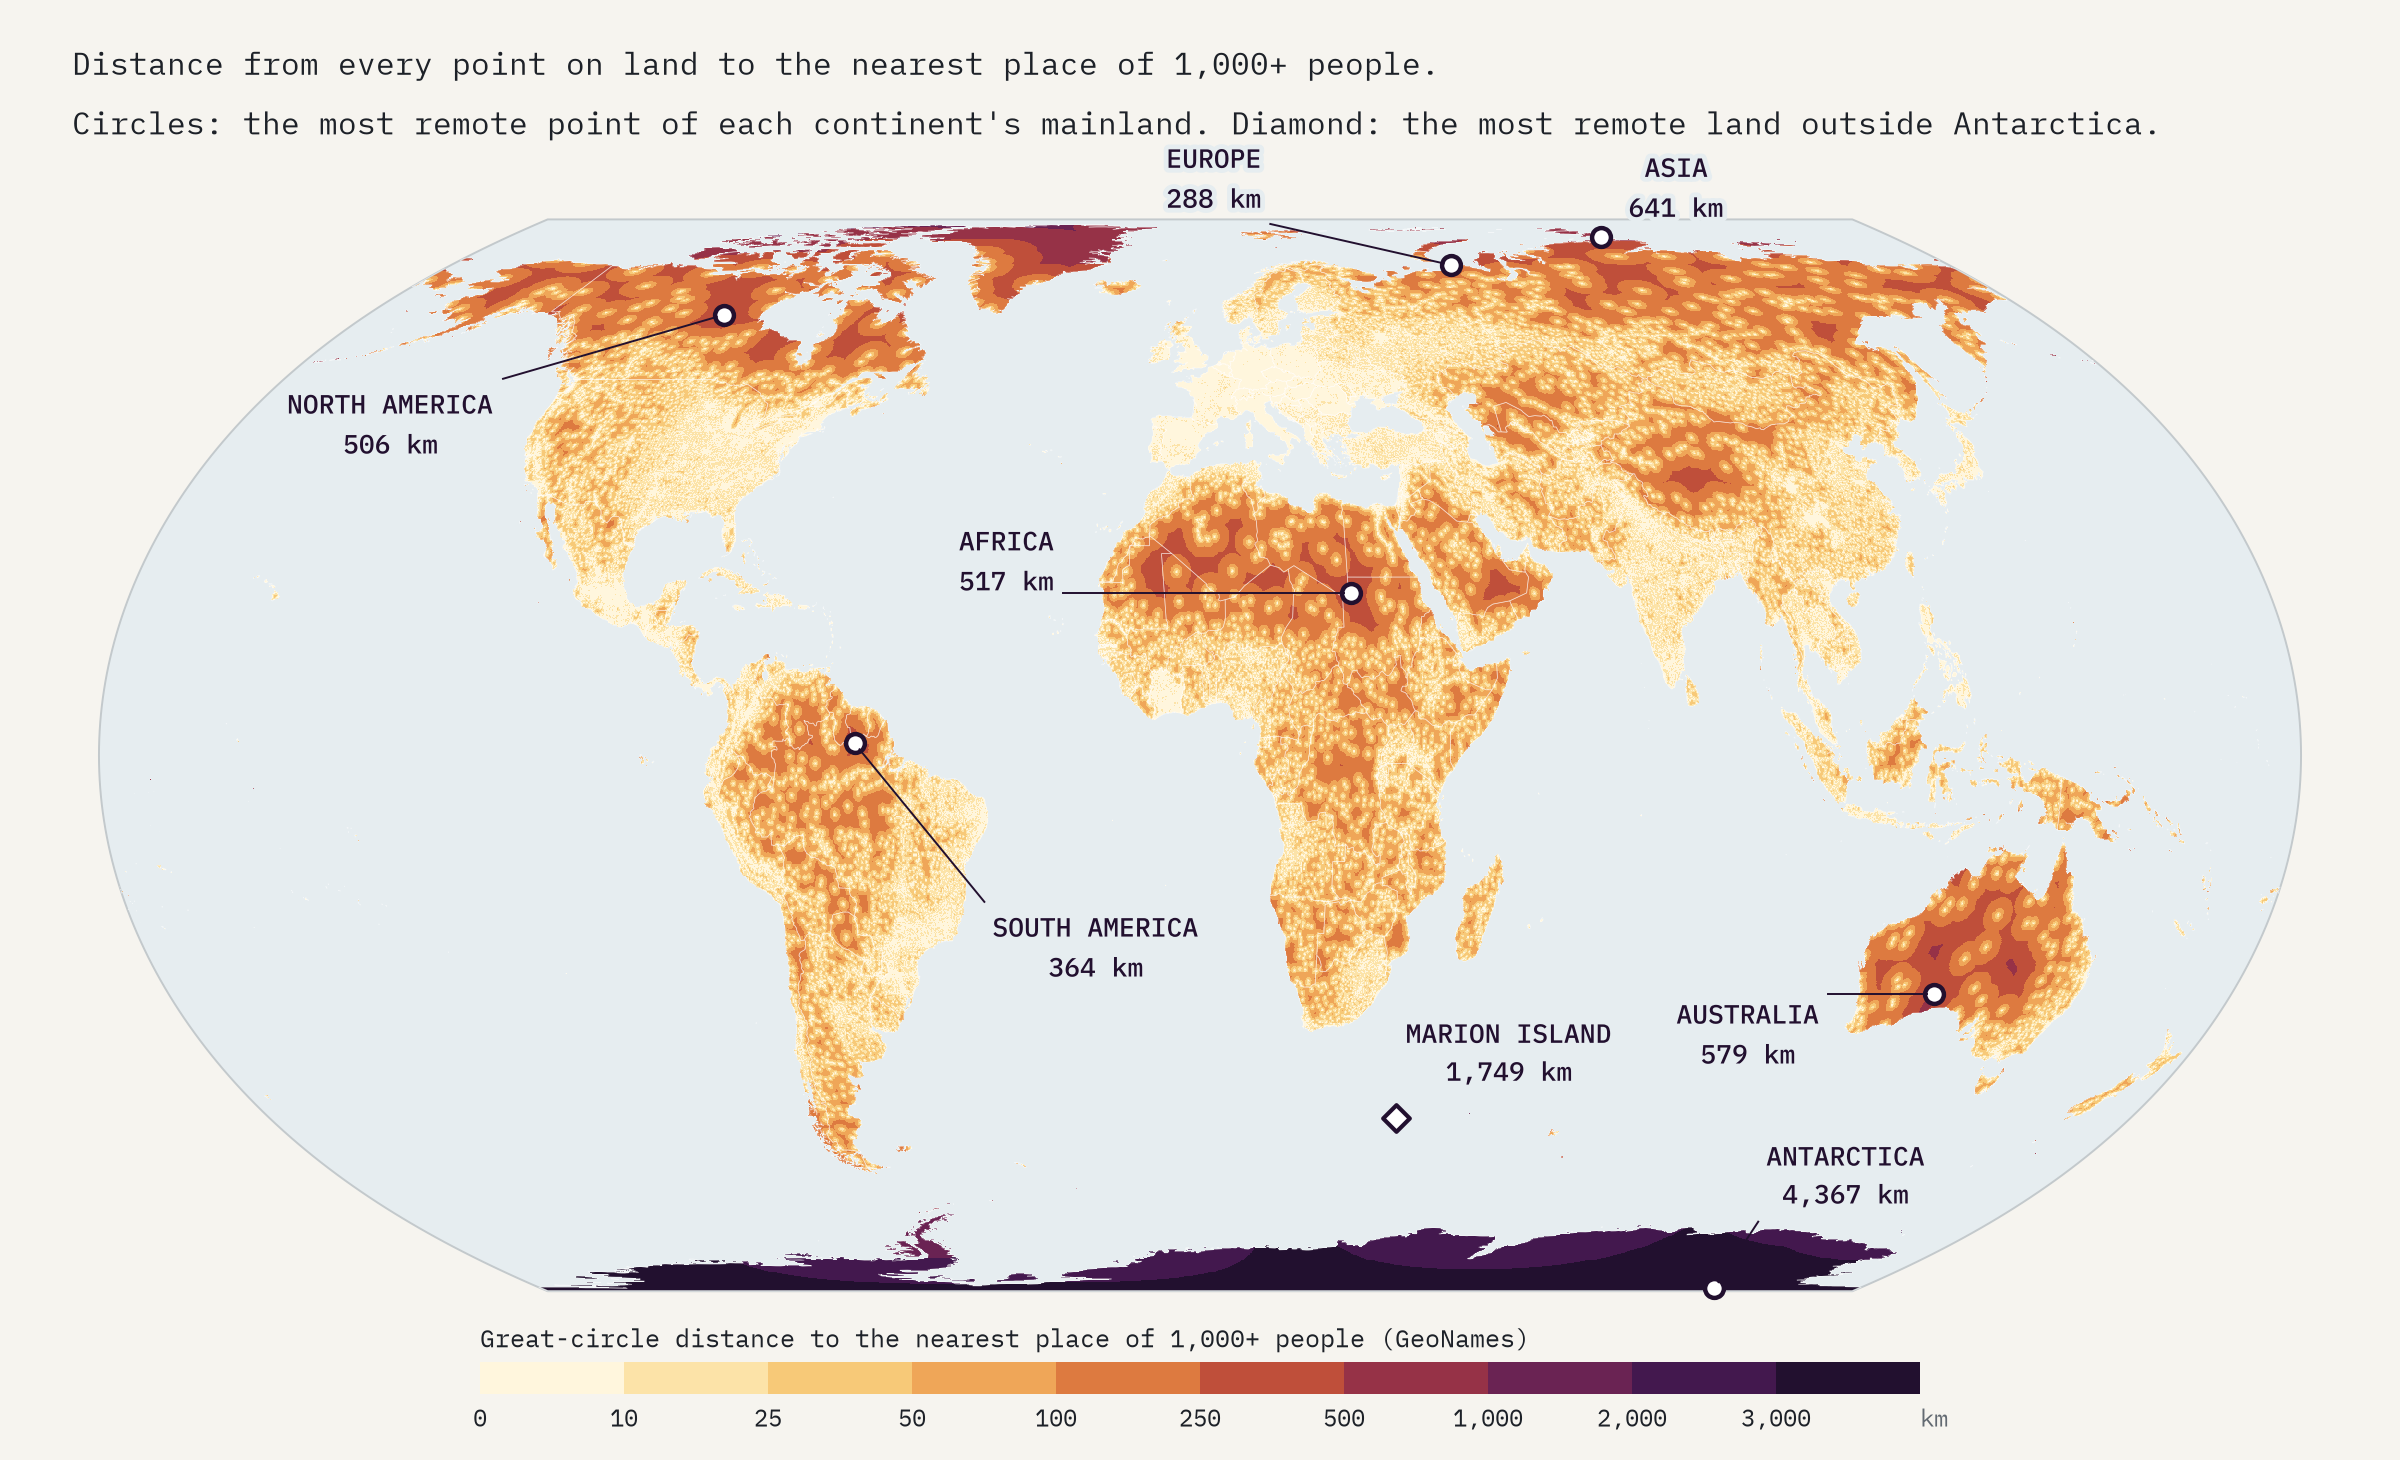
\includegraphics[width=\textwidth]{f_map_town.png}
\caption{Distance from every point on land to the nearest place of 1,000 or more people, with the most remote point of each continent's mainland and of all land outside Antarctica (Marion Island). Equal Earth projection.}\label{fig:map}\end{figure}

\begin{figure}[tbp]\centering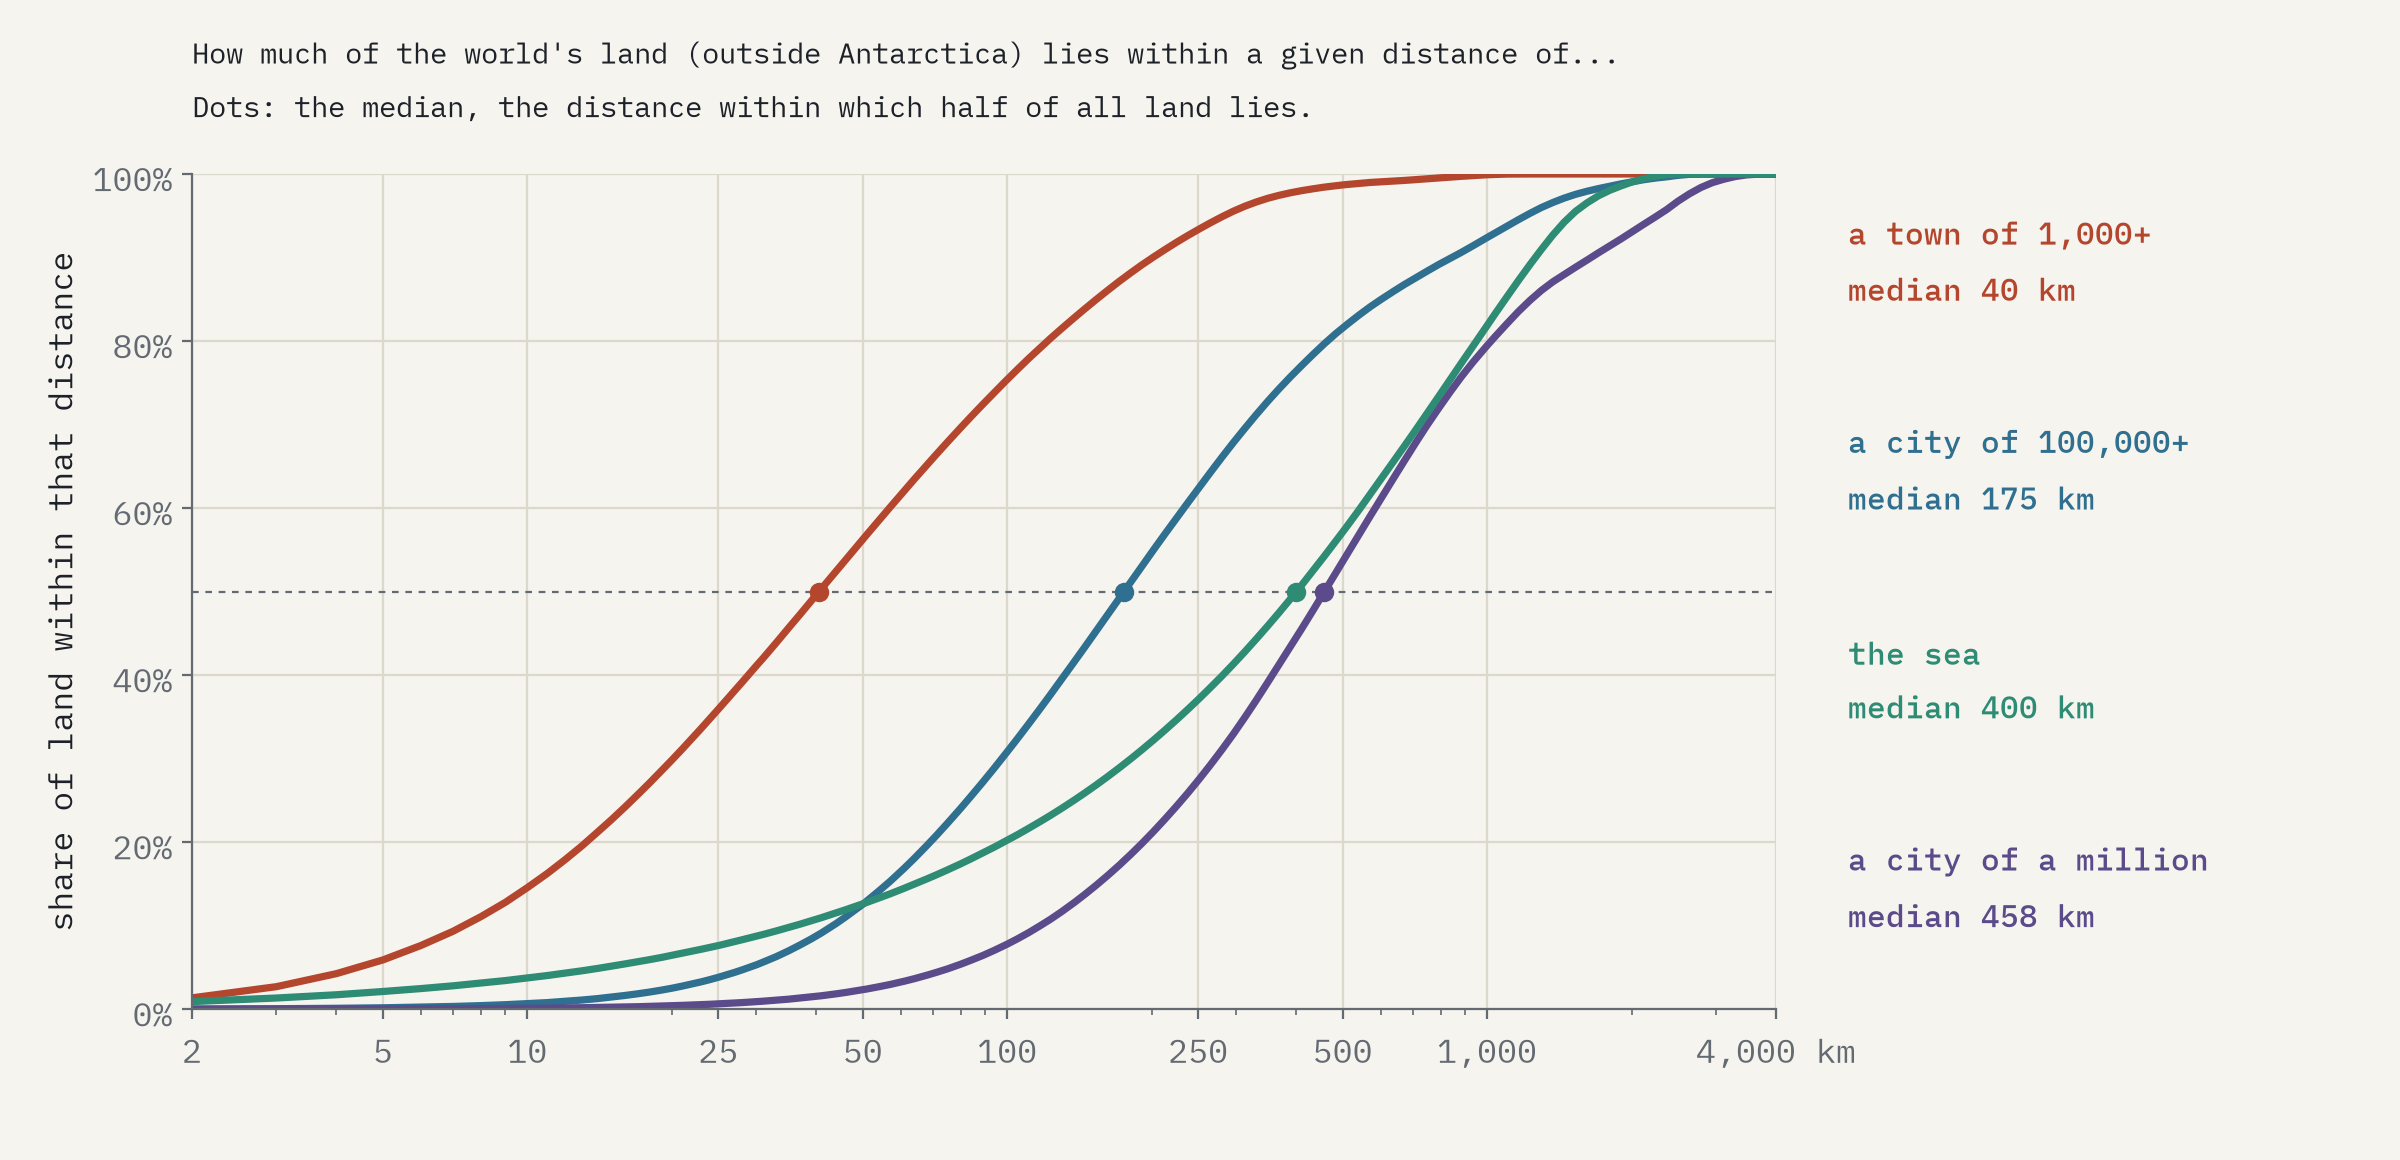
\includegraphics[width=\textwidth]{f_share.png}
\caption{Cumulative share of the land outside Antarctica within a given distance of a town, a city of 100,000+, a city of a million and the coast. Dots mark the medians.}\label{fig:share}\end{figure}

Remoteness is concentrated at high northern latitudes and in the subtropical deserts (Figure~\ref{fig:lat}). Land north of 60\textdegree N is 12.8\% of the land outside Antarctica but holds 34.9\% of the land more than 100 km from a town and 93.2\% of that more than 500 km away.

\begin{figure}[tbp]\centering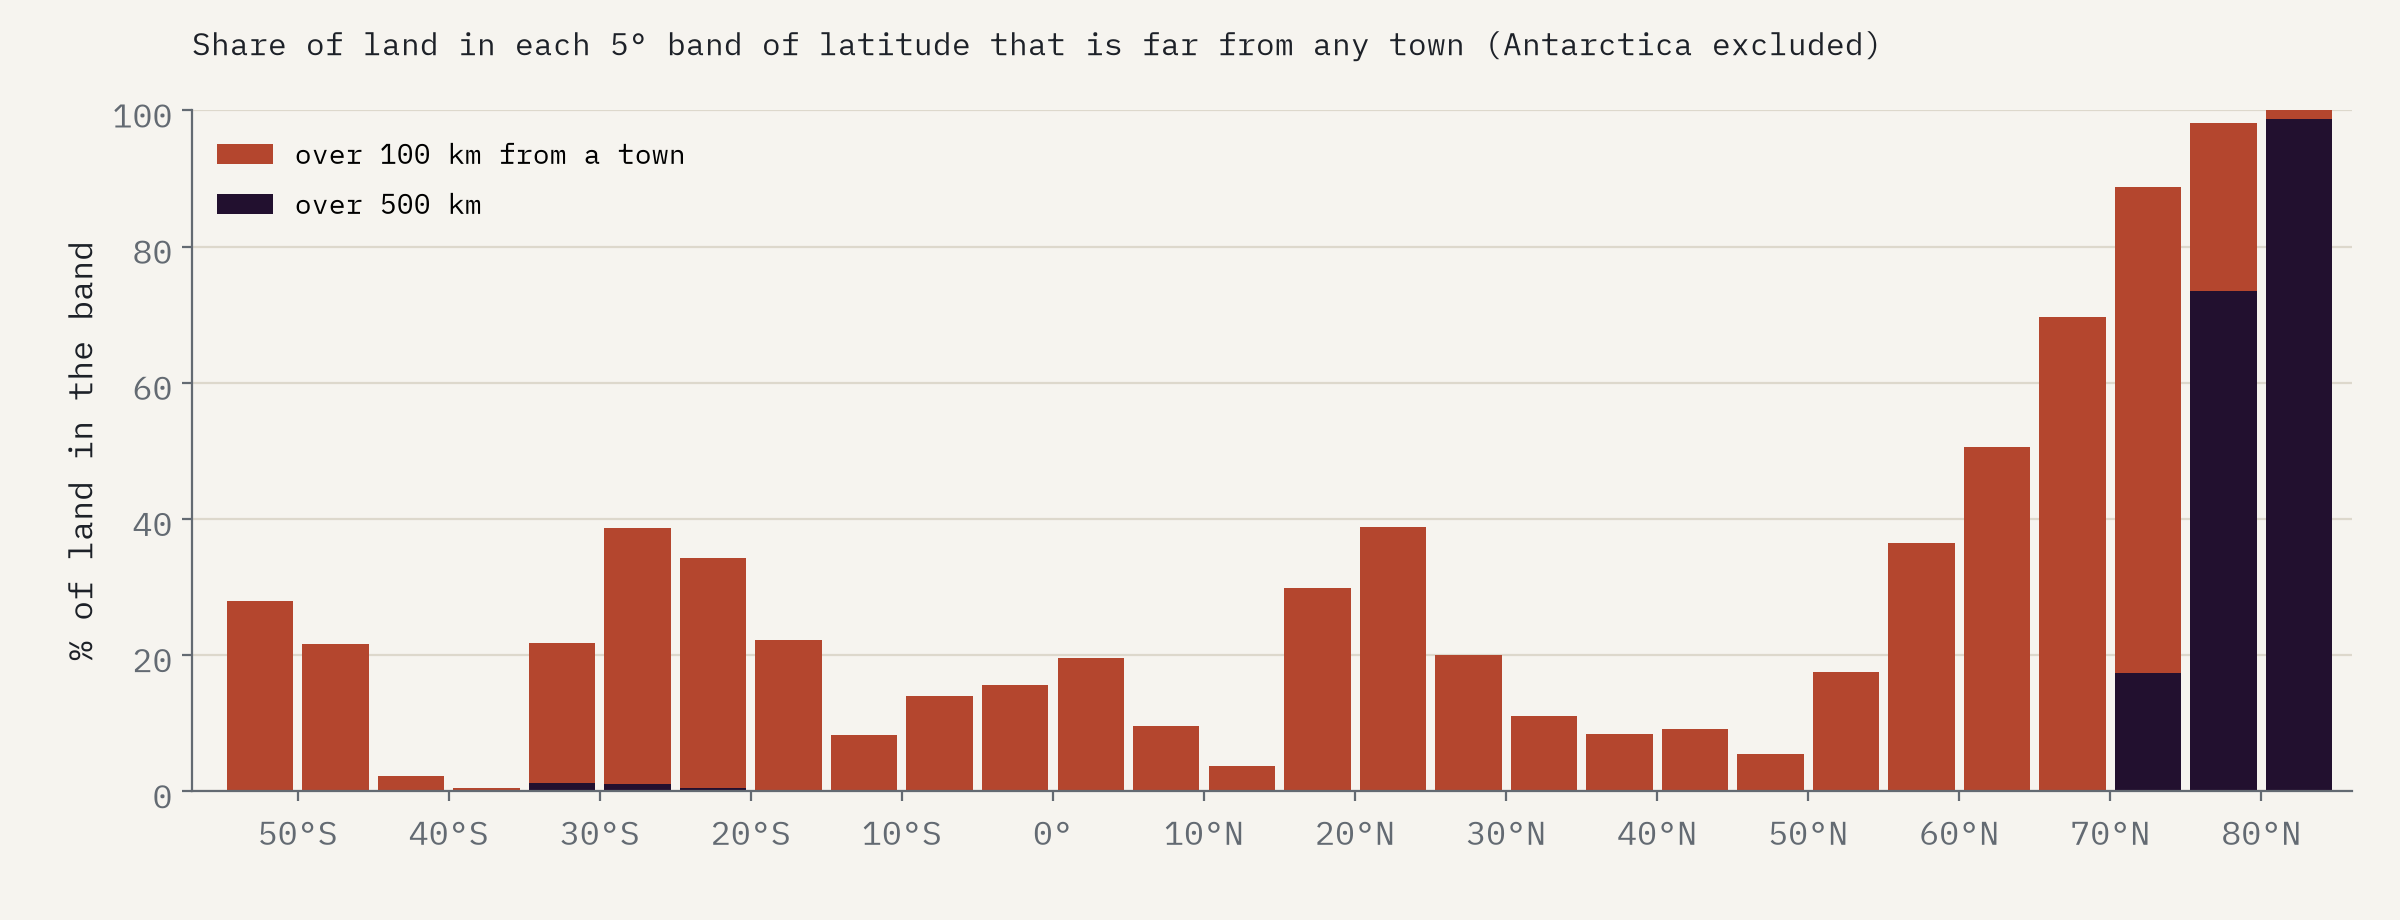
\includegraphics[width=\textwidth]{f_lat.png}
\caption{Share of land in each 5\textdegree{} band of latitude more than 100 km and more than 500 km from a town.}\label{fig:lat}\end{figure}

\subsection{Continents and islands}
Table~\ref{tab:cont} and Figure~\ref{fig:cont} give the most remote point of each mainland for the four measures. From a town, Asia's lies at Cape Chelyuskin on the Taymyr Peninsula, Australia's in the Great Victoria Desert of Western Australia, Africa's in the Libyan Desert of north-western Sudan, North America's in the far north of Saskatchewan, South America's in the forest of northern Par\'a near Suriname, and Europe's on the Kara Sea coast of north-eastern European Russia. The far-from-the-sea maxima fall close to the published continental poles of inaccessibility: in the Central African Republic near Obo, in South Dakota, in Mato Grosso and west of Alice Springs. The Eurasian maximum, at 45.83\textdegree{}N 88.76\textdegree{}E and 2,478 km from the coast, lies 169 km from the commonly cited position of about 46\textdegree 17$'$N 86\textdegree 40$'$E, where my coastline gives 2,382 km; the difference reflects the generalised 1:50m coastline and the treatment of the Caspian and Arctic shores. Both points are less than 100 km from a town (65 km and 57 km).

\begin{table}[tbp]\centering\footnotesize\setlength{\tabcolsep}{4pt}\caption{The most remote point of each mainland: km to the nearest town, its position and the town; km from the most remote points for cities of 100,000+ and 1,000,000+ and for the coast, with the position of the coast maximum.}\label{tab:cont}\resizebox{\textwidth}{!}{\begin{tabular}{lrllrrrl}\toprule Mainland & Town & Where & Nearest town & 100k & 1m & Coast & Where\\\midrule
Africa & 517 & 20.01N 25.49E & Karmah an Nuzul & 977 & 1,430 & 1,820 & 5.71N 26.15E\\
Asia & 641 & 77.73N 104.18E & Khatanga & 1,994 & 3,655 & 2,478 & 45.83N 88.76E\\
Europe & 288 & 69.85N 60.35E & Vorgashor & 732 & 1,445 & 1,192 & 57.28N 57.66E\\
North America & 506 & 59.72N 102.84W & Fort Smith & 2,310 & 3,170 & 1,642 & 43.36N 102.05W\\
South America & 364 & 1.45N 56.47W & Oriximiná & 798 & 2,272 & 1,498 & 14.34S 56.97W\\
Australia & 579 & 29.84S 128.21E & Ceduna & 1,583 & 2,170 & 934 & 23.16S 132.31E\\
Antarctica & 4,367 & 85.29S 140.56E & Puerto Williams & 5,291 & 6,000 & 1,139 & 77.38S 105.48E\\
\bottomrule\end{tabular}}\end{table}

\begin{figure}[tbp]\centering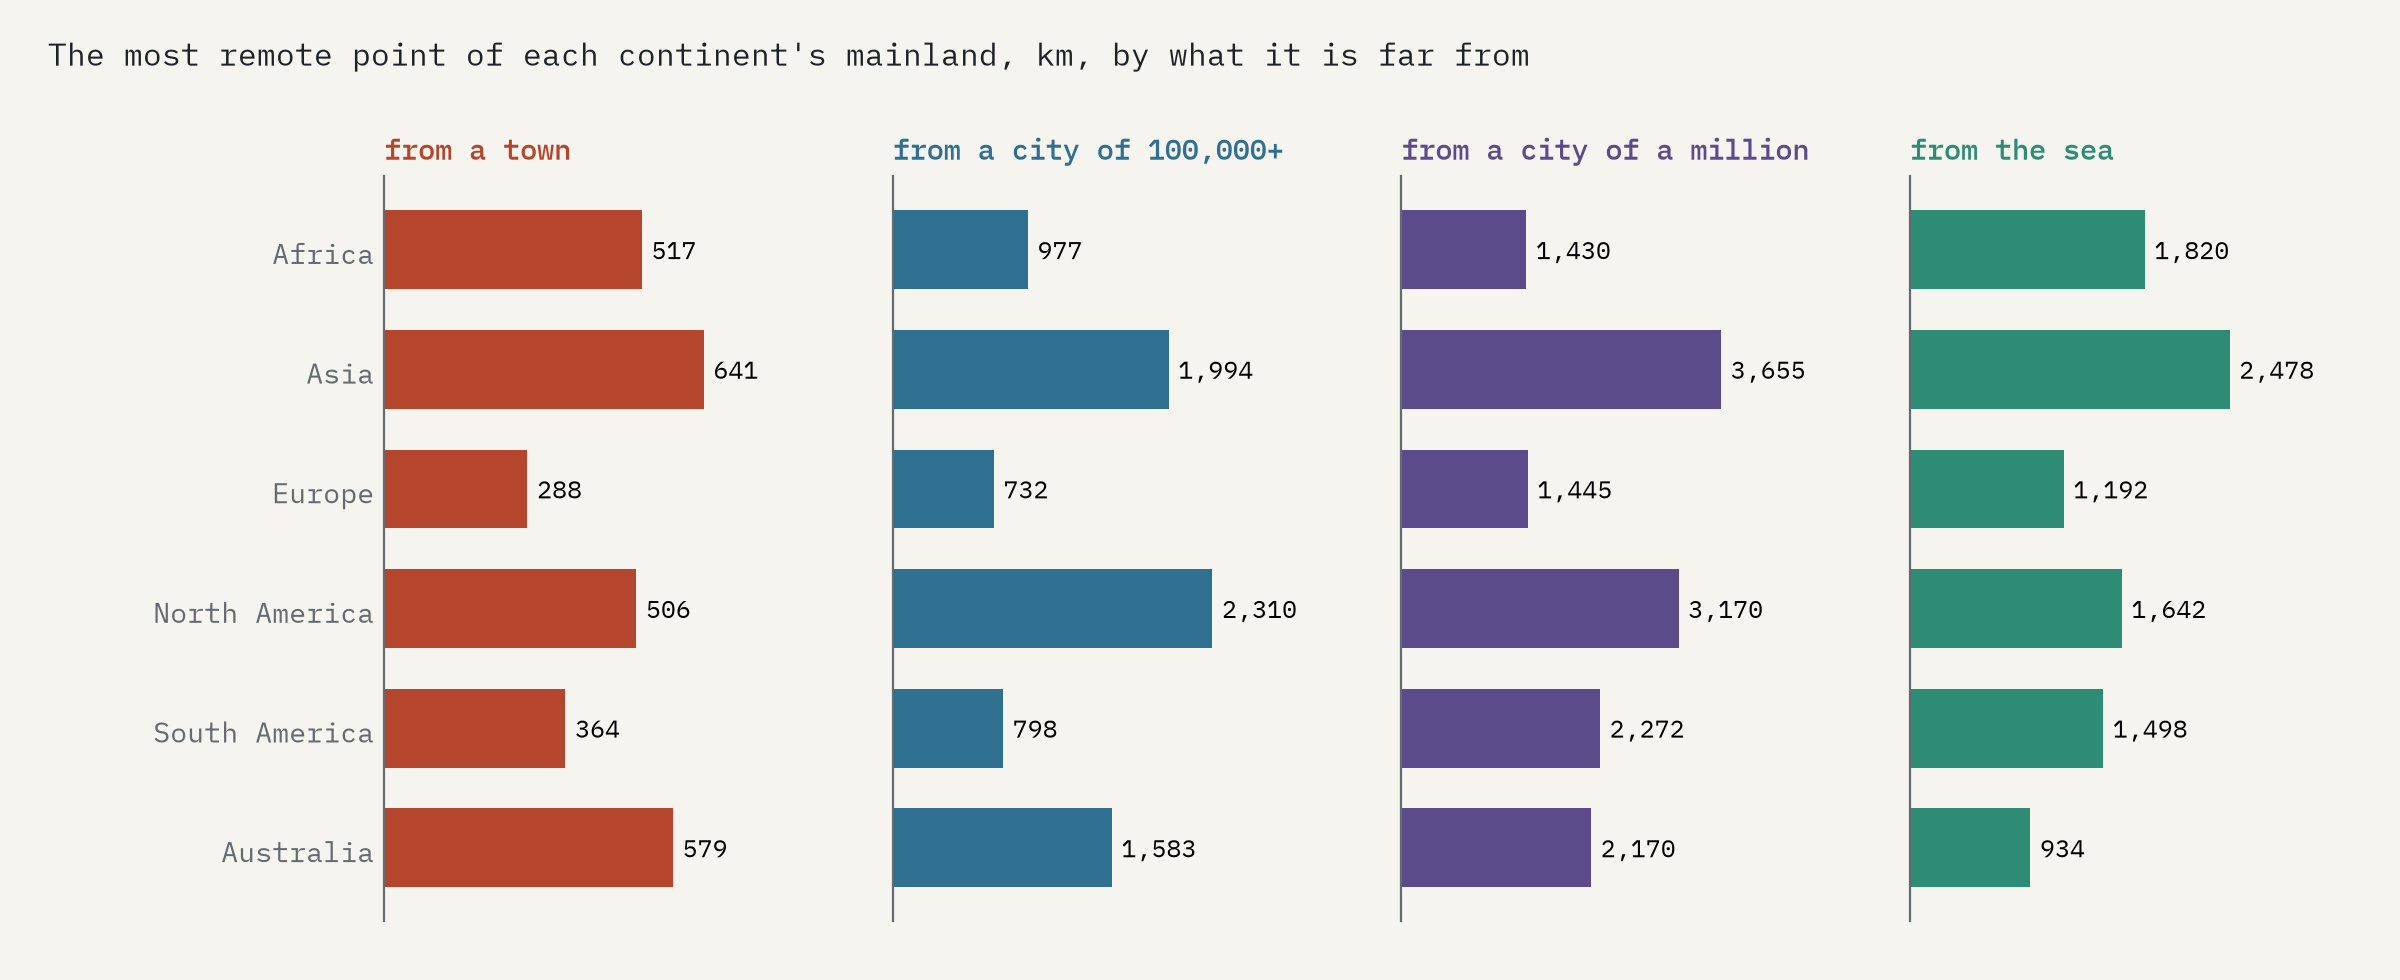
\includegraphics[width=\textwidth]{f_continents.png}
\caption{The most remote point of each continent's mainland, km, for each measure.}\label{fig:cont}\end{figure}

Islands hold the global maxima. Outside Antarctica the land farthest from a town is Marion Island in the Prince Edward Islands (1,749 km from Port Alfred), followed by the Crozet Islands (1,419 km from Port-aux-Français, the base on Kerguelen, which GeoNames lists as an administrative seat). In the Arctic, Cape Columbia on Ellesmere Island is 1,170 km from a town and the north coast of Greenland 1,162 km; 93\% of Greenland is more than 100 km from one (Table~\ref{tab:isl}). For cities, the most remote land is Heard Island (3,905 km from a city of 100,000) and the Marquesas Islands (5,231 km from a city of a million).

\begin{table}[tbp]\centering\small\caption{The fifteen largest islands: grid area, the most remote point from a town and the share of the island more than 100 km from one.}\label{tab:isl}\begin{tabular}{lrrllr}\toprule Island & km\textsuperscript{2} & km to town & Where & Nearest town & Over 100 km\\\midrule
Ellesmere Island & 201,308 & 1,170 & 83.11N 69.88W & Pond Inlet & 100.0\%\\
Greenland & 2,146,304 & 1,162 & 83.06N 46.17W & Longyearbyen & 93.0\%\\
Victoria Island & 219,832 & 593 & 73.16N 115.89W & Cambridge Bay & 92.1\%\\
Baffin Island & 519,526 & 415 & 71.94N 90.02W & Igloolik & 82.9\%\\
New Guinea & 786,917 & 181 & 7.50S 142.74E & Mendi & 8.2\%\\
Borneo & 735,775 & 161 & 0.66S 113.14E & Nangah Pinoh & 6.0\%\\
Iceland & 103,176 & 135 & 64.47N 17.98W & Akureyri & 9.7\%\\
Madagascar & 597,369 & 122 & 20.63S 45.55E & Ikalamavony & 0.5\%\\
South Island, New Zealand & 152,739 & 112 & 45.95S 166.49E & Te Anau & 0.2\%\\
Tasmania & 64,568 & 105 & 43.03S 145.64E & Geeveston & 0.0\%\\
Sulawesi & 173,523 & 100 & 1.59S 122.15E & Luwuk & 0.0\%\\
Sumatra & 431,193 & 95 & 3.01S 105.70E & Sungaigerong & 0.0\%\\
Great Britain & 219,767 & 78 & 58.58N 4.87W & Ullapool & 0.0\%\\
Ireland & 85,734 & 40 & 51.61N 10.03W & Cahersiveen & 0.0\%\\
Honshu & 230,296 & 34 & 36.04N 136.88E & Katsuyama & 0.0\%\\
\bottomrule\end{tabular}\end{table}

\subsection{Famous empty places}
Table~\ref{tab:cand} checks regions often named as the world's emptiest. The Sahara's most remote point from a town is 517 km away and 60\% of the box drawn around it is more than 100 km from one; Tibet's Changtang reaches 426 km, the Empty Quarter 407 km, the Australian interior 579 km and mainland Siberia 641 km, while the Amazon reaches 364 km. The Arctic islands of Canada and Greenland exceed them all.

\begin{table}[tbp]\centering\small\caption{Famous empty places: the most remote point from a town within each region and the share of the region more than 100 km from one. Regions are boxes or countries (see code/common.py).}\label{tab:cand}\resizebox{\textwidth}{!}{\begin{tabular}{lrllr}\toprule Region & km to town & Where & Nearest town & Over 100 km\\\midrule
Sahara & 517 & 20.01N 25.49E & Karmah an Nuzul (Sudan) & 59.6\%\\
Rub' al Khali (Empty Quarter) & 407 & 21.11N 50.45E & Rumāh (Yemen) & 58.7\%\\
Tibet's Changtang & 426 & 34.90N 88.17E & Pubu (China) & 70.9\%\\
Australian interior & 579 & 29.84S 128.21E & Ceduna (Australia) & 61.6\%\\
Greenland & 1,162 & 83.06N 46.17W & Longyearbyen (Svalbard (Norway)) & 92.8\%\\
Northern Canada (north of 60 N) & 1,170 & 83.11N 69.88W & Pond Inlet (Canada) & 84.1\%\\
Siberia (mainland Russia east of 60 E) & 641 & 77.73N 104.18E & Khatanga (Russia) & 48.3\%\\
Amazon (Brazil) & 364 & 1.45N 56.47W & Oriximiná (Brazil) & 14.7\%\\
\bottomrule\end{tabular}}\end{table}

\subsection{Antarctica}
Antarctica's research stations are not in the gazetteer, so on this measure the continent has no towns at all. Every point of it is at least 879 km from a town, its median distance is 3,180 km, and its most remote point, on the polar plateau at 85.29\textdegree{}S 140.56\textdegree{}E, is 4,367 km from Puerto Williams. Its farthest point from the Natural Earth coast is 1,139 km inland at 77.38\textdegree{}S 105.48\textdegree{}E; because the outline excludes the floating ice shelves, this differs from calculations that use the ice front as the coast.

\subsection{Countries}
Counting islands, the countries with the most remote points are South Africa (Marion Island), Canada (Ellesmere Island), Greenland, the United States (the western Aleutian Islands, whose nearest town is Nikol’skoye in Russia) and Russia (Franz Josef Land). On each country's main land mass the order is Greenland, Russia, Australia, Sudan and Canada (Table~\ref{tab:cty}, Figure~\ref{fig:cty}). For 34 countries the nearest town to the most remote point is in another country. The median country's most remote point is 72 km from a town, and 23 small countries have no point more than 10 km from one.

\begin{figure}[tbp]\centering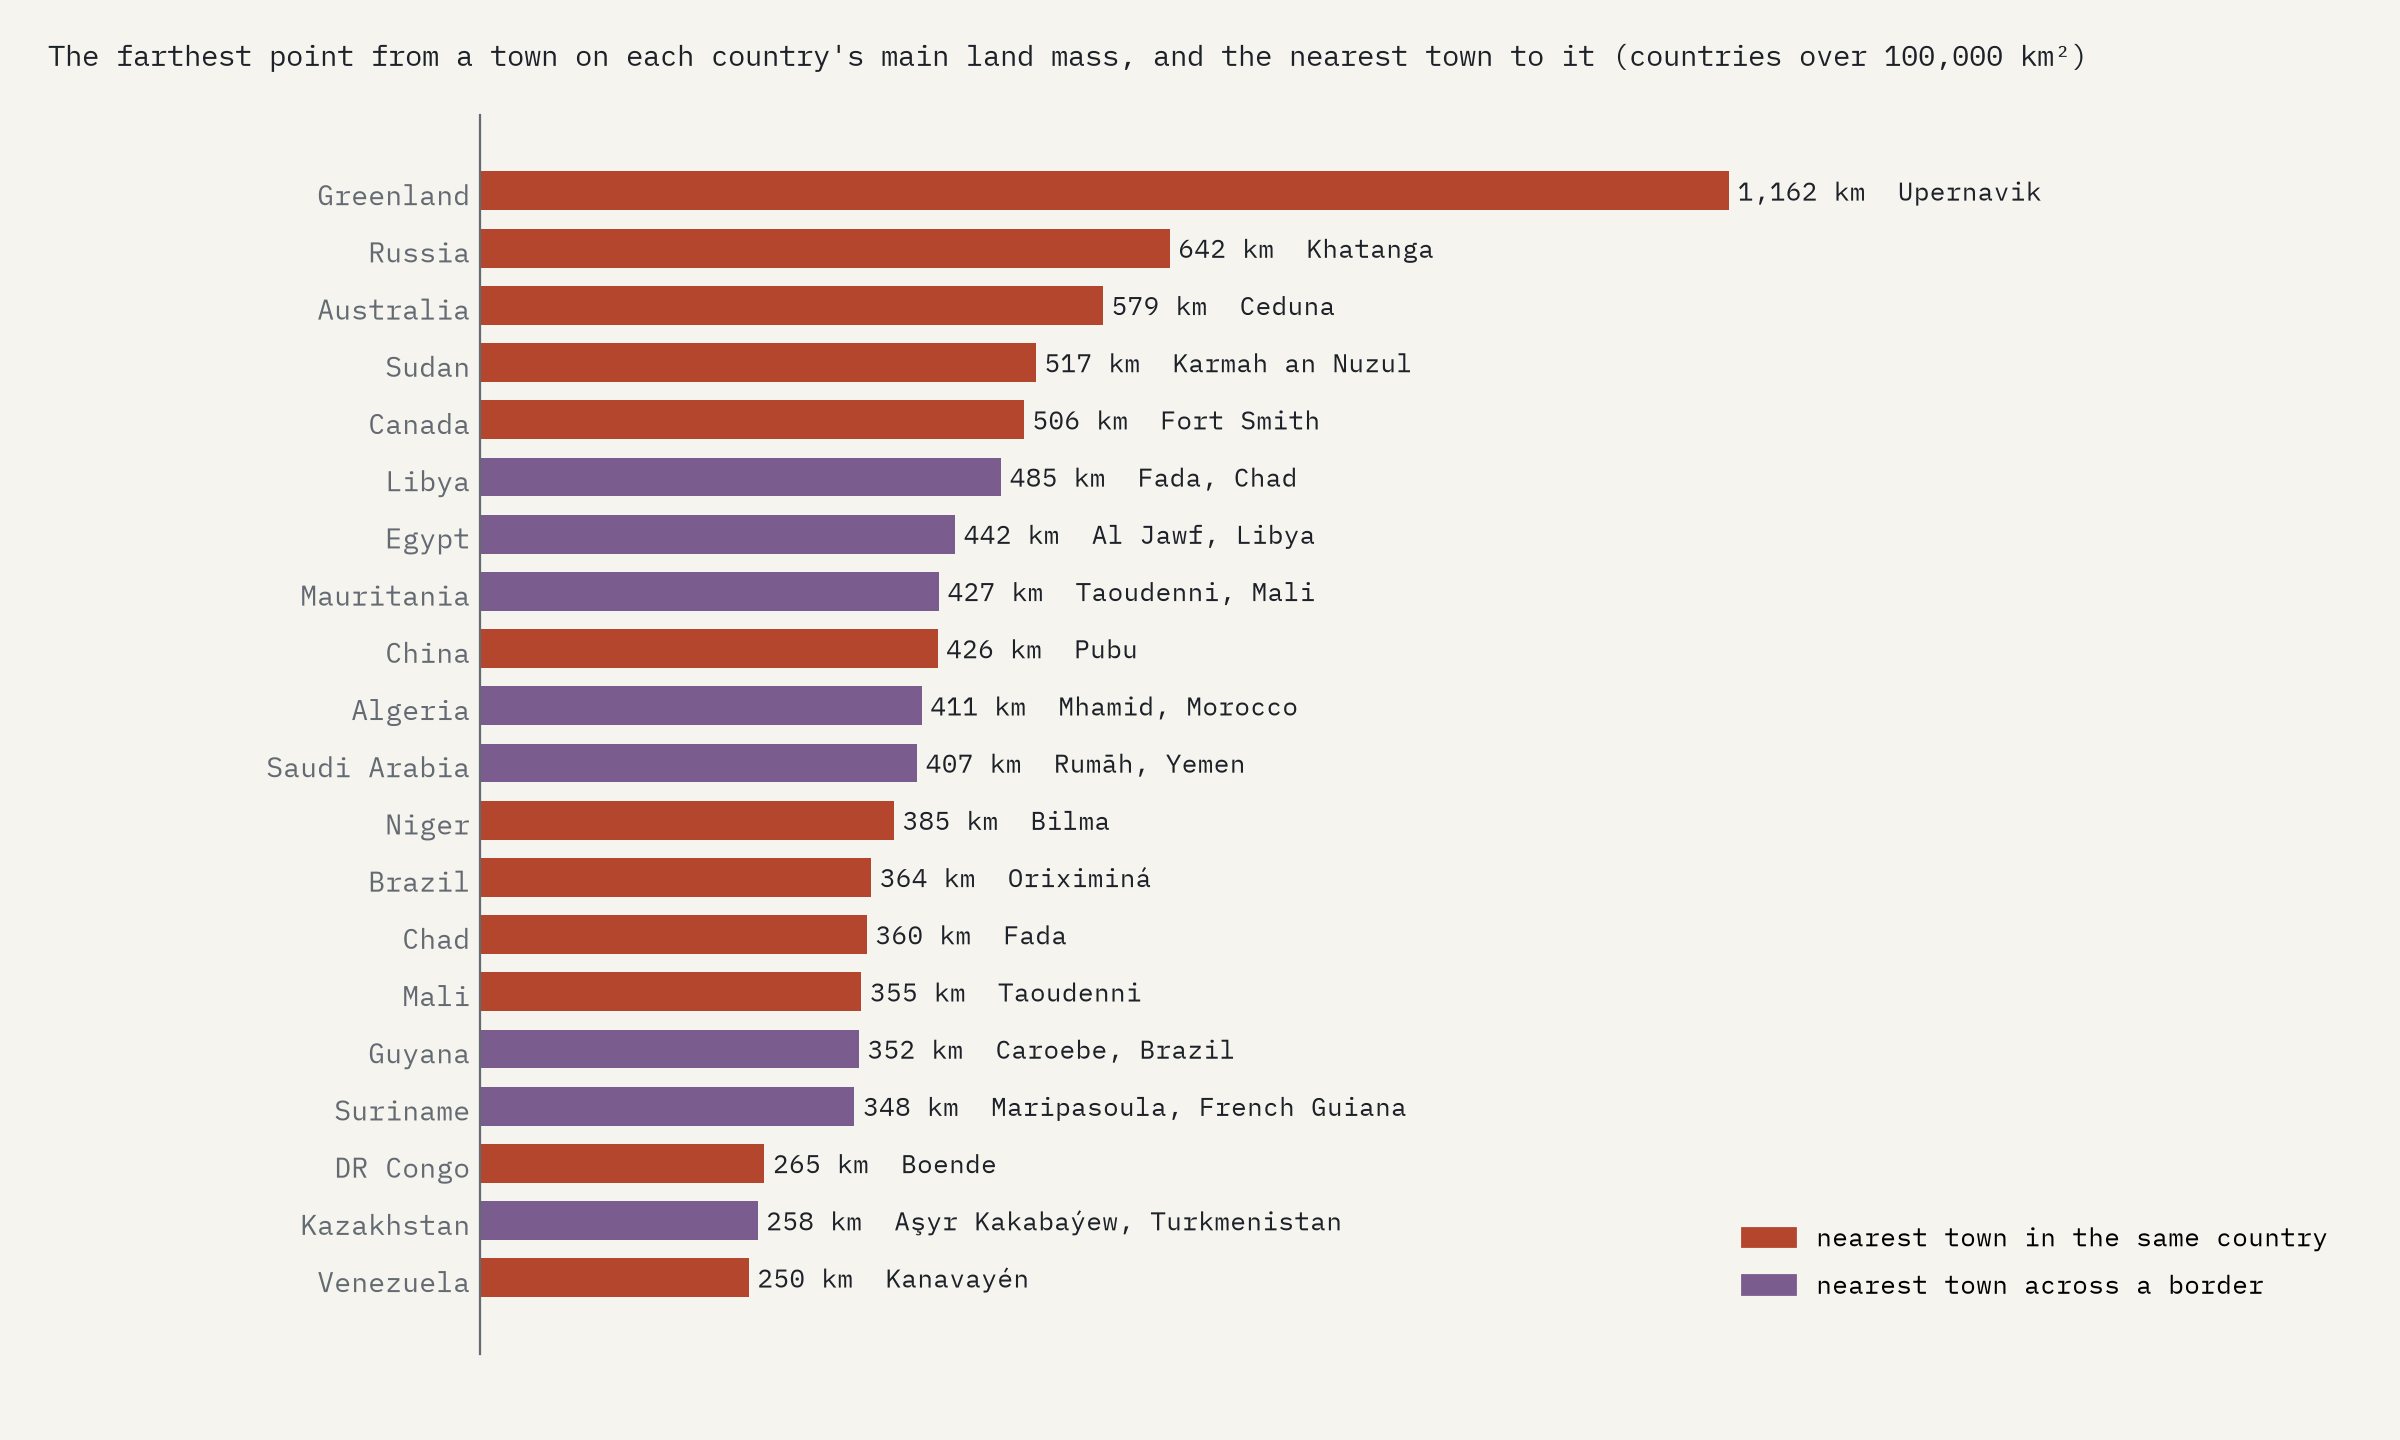
\includegraphics[width=\textwidth]{f_countries.png}
\caption{The farthest point from a town on the main land mass of each country over 100,000 km\textsuperscript{2}; purple: the nearest town is in another country.}\label{fig:cty}\end{figure}

\begin{table}[tbp]\centering\footnotesize\caption{The 25 countries over 100,000 km\textsuperscript{2} whose main land mass reaches farthest from a town: km, position and nearest town (country if different); km counting all islands; share of the country more than 100 km from a town. All countries and territories are in data/country\_remote\_points.csv.}\label{tab:cty}\resizebox{\textwidth}{!}{\begin{tabular}{lrllrr}\toprule Country & km & Where & Nearest town & With islands & Over 100 km\\\midrule
Greenland & 1,162 & 83.06N 46.19W & Upernavik & 1,162 & 92.8\%\\
Russia & 642 & 77.73N 104.32E & Khatanga & 974 & 38.6\%\\
Australia & 579 & 29.84S 128.21E & Ceduna & 579 & 60.9\%\\
Sudan & 517 & 20.01N 25.49E & Karmah an Nuzul & 517 & 45.8\%\\
Canada & 506 & 59.72N 102.84W & Fort Smith & 1,171 & 58.7\%\\
Libya & 485 & 20.13N 24.98E & Fada (Chad) & 485 & 60.4\%\\
Egypt & 442 & 22.00N 26.89E & Al Jawf (Libya) & 442 & 43.6\%\\
Mauritania & 427 & 23.01N 8.13W & Taoudenni (Mali) & 427 & 48.2\%\\
China & 426 & 34.90N 88.17E & Pubu & 426 & 16.2\%\\
Algeria & 411 & 26.37N 4.22W & Mhamid (Morocco) & 411 & 59.0\%\\
Saudi Arabia & 407 & 21.11N 50.45E & Rumāh (Yemen) & 407 & 38.6\%\\
Niger & 385 & 22.12N 12.45E & Bilma & 385 & 48.1\%\\
Brazil & 364 & 1.45N 56.47W & Oriximiná & 364 & 14.7\%\\
Chad & 360 & 19.50N 23.97E & Fada & 360 & 38.9\%\\
Mali & 355 & 24.81N 6.57W & Taoudenni & 355 & 39.4\%\\
Guyana & 352 & 1.92N 56.70W & Caroebe (Brazil) & 352 & 42.6\%\\
Suriname & 348 & 2.15N 56.79W & Maripasoula (French Guiana) & 348 & 56.5\%\\
DR Congo & 265 & 1.19S 23.08E & Boende & 265 & 26.1\%\\
Kazakhstan & 258 & 42.13N 55.59E & Aşyr Kakabaýew (Turkmenistan) & 258 & 15.0\%\\
Venezuela & 250 & 4.61N 63.81W & Kanavayén & 250 & 18.4\%\\
Chile & 247 & 46.64S 75.70W & Cochrane & 628 & 18.1\%\\
Mongolia & 240 & 42.75N 97.58E & Dzalaa & 240 & 4.8\%\\
Colombia & 236 & 0.77S 69.61W & Mitú & 236 & 17.6\%\\
Central African Republic & 235 & 6.94N 24.20E & Ouadda & 235 & 18.2\%\\
Uzbekistan & 233 & 41.78N 55.98E & Aşyr Kakabaýew (Turkmenistan) & 233 & 25.4\%\\
\bottomrule\end{tabular}}\end{table}

\begin{figure}[tbp]\centering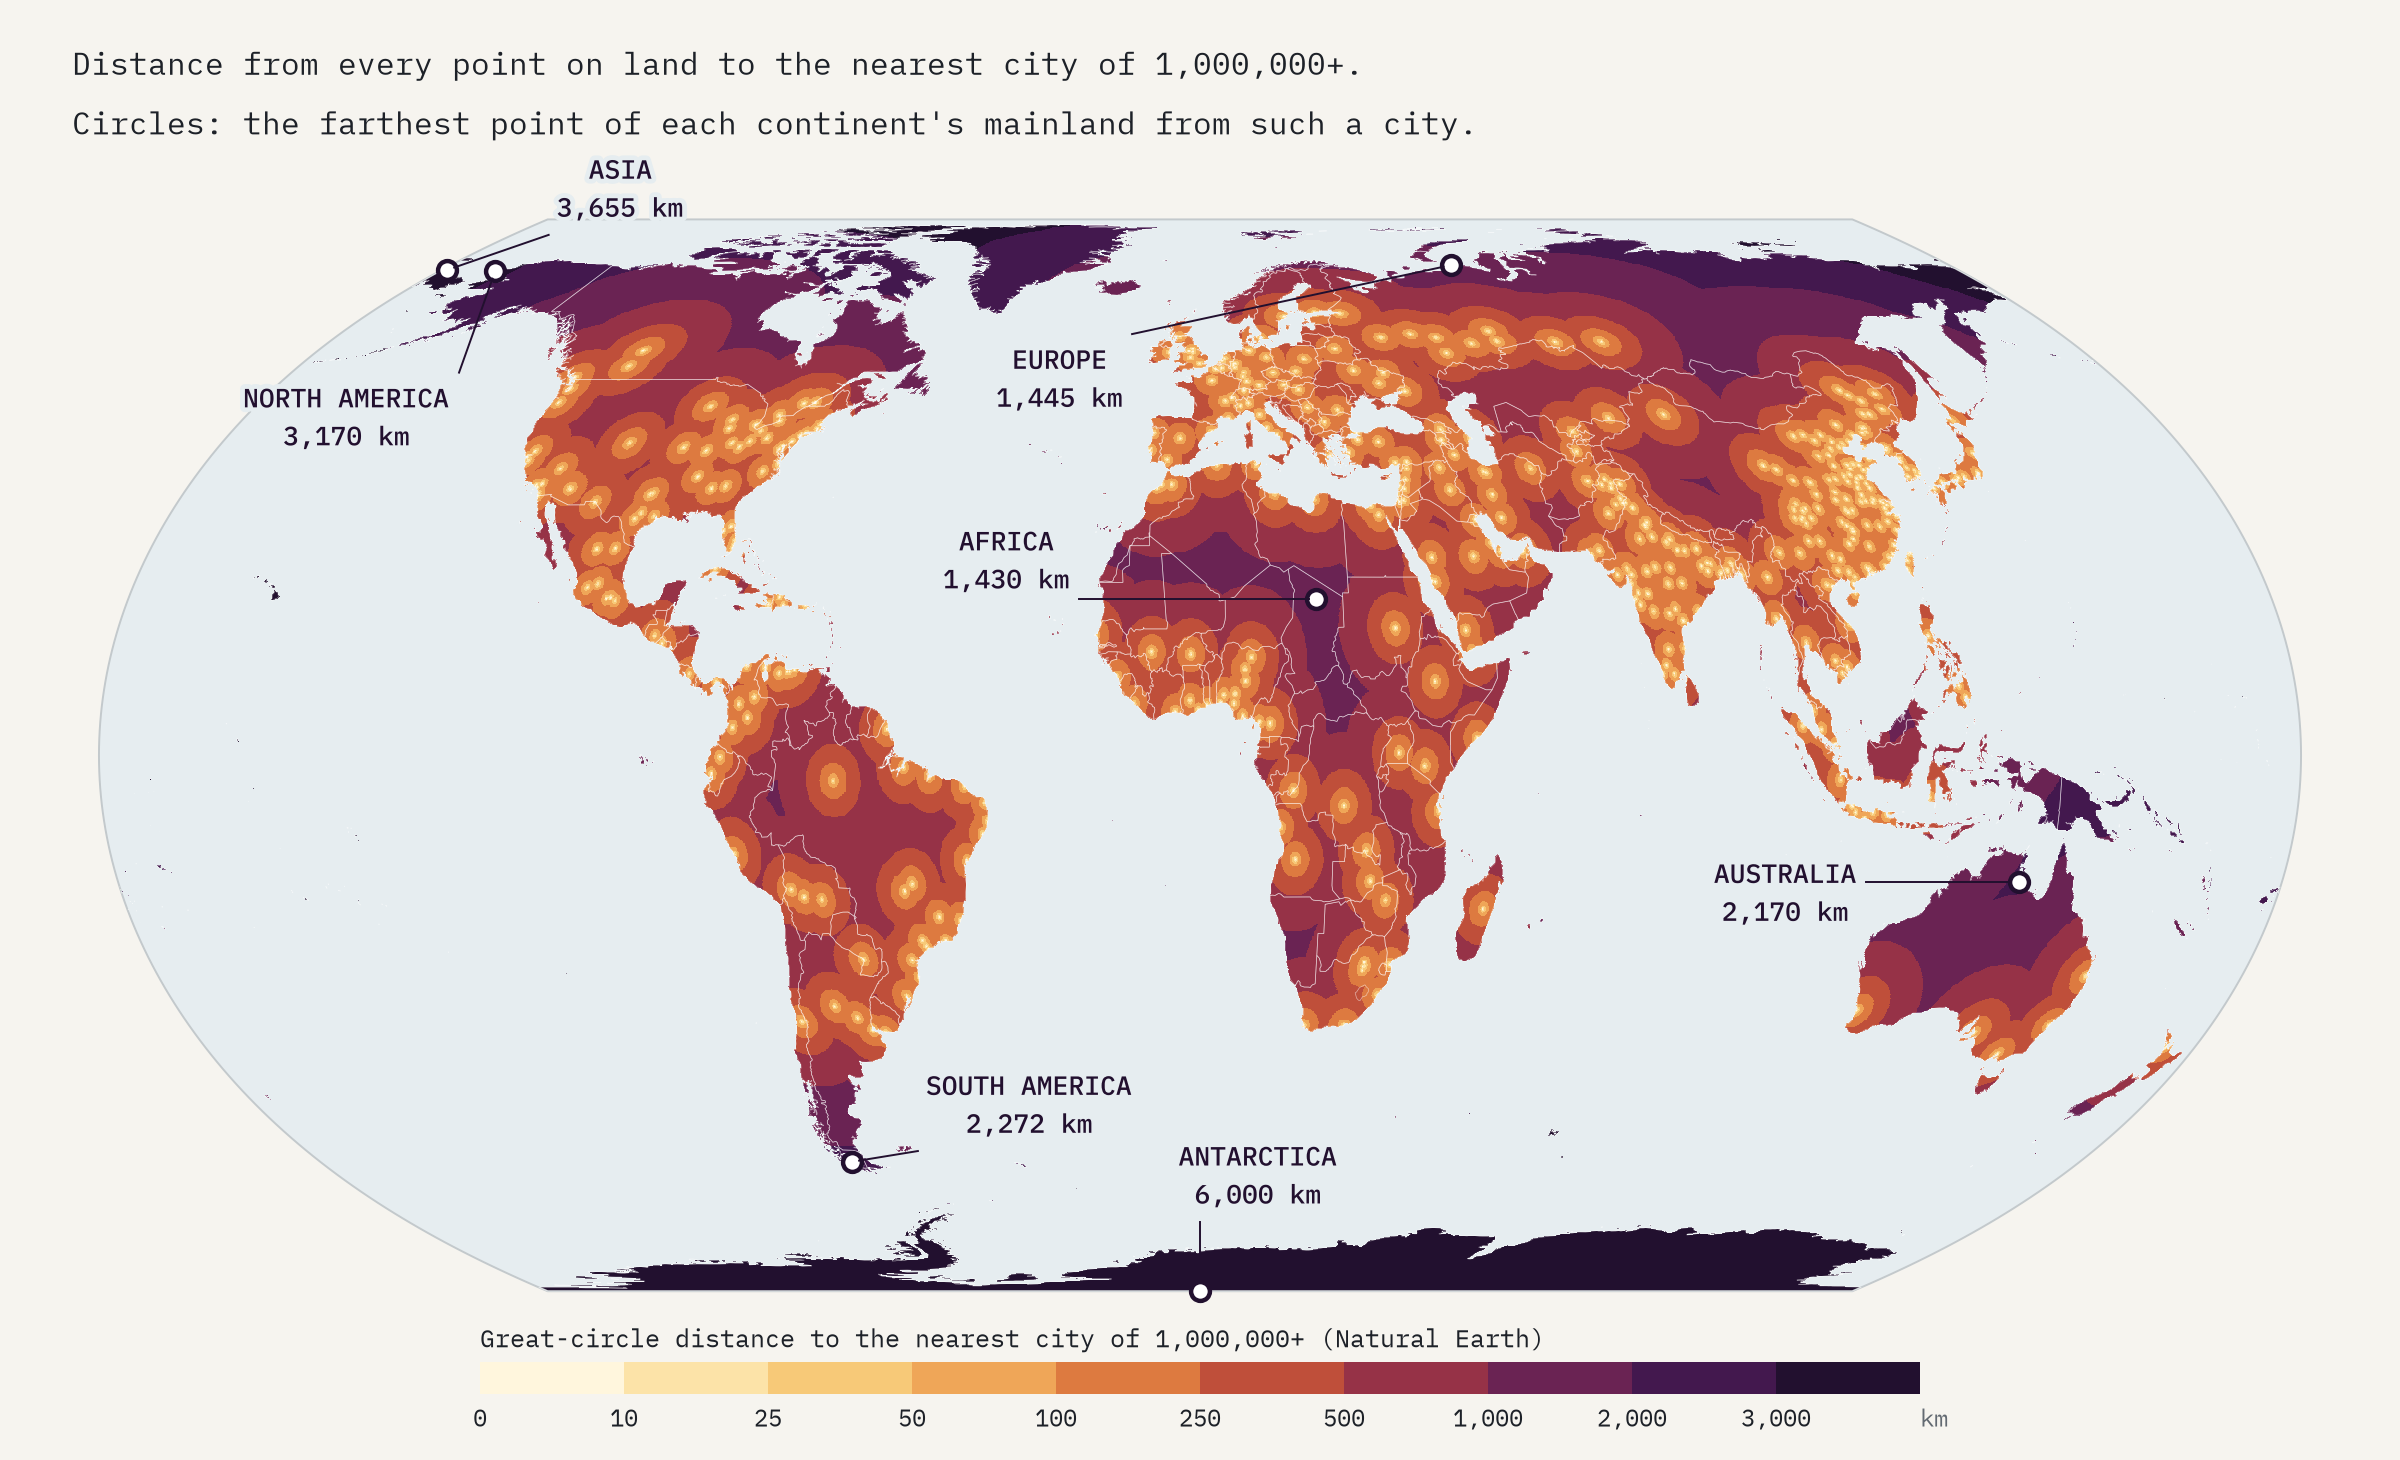
\includegraphics[width=\textwidth]{f_map_c1m.png}
\caption{Distance from every point on land to the nearest city of 1,000,000 or more, with the farthest point of each continent's mainland.}\label{fig:c1m}\end{figure}

\subsection{The United Kingdom}
In a densely settled country the same measure works in tens of kilometres (Figure~\ref{fig:uk}). Half of the island of Great Britain is within 4.2 km of a town and 20.6\% is more than 10 km from one. The most remote spot on the island is near Cape Wrath at 58.62\textdegree{}N 4.96\textdegree{}W, 82 km from Ullapool, and most of the ten most remote spots, at least 30 km apart, are in the Highland council area. 52.7\% of mainland Scotland is more than 10 km from a town, against 3.4\% of England and 10.3\% of Wales. England's most remote point is in Kielder Forest, Northumberland (24 km, nearest town Langholm in Scotland), or Lundy if islands count (36 km); Wales's is the tip of the Ll\^yn Peninsula (23 km) and Northern Ireland's is in the Sperrin Mountains (20 km). On a small, busy island, the ends of peninsulas are often farther from a town than the uplands.

\begin{figure}[tbp]\centering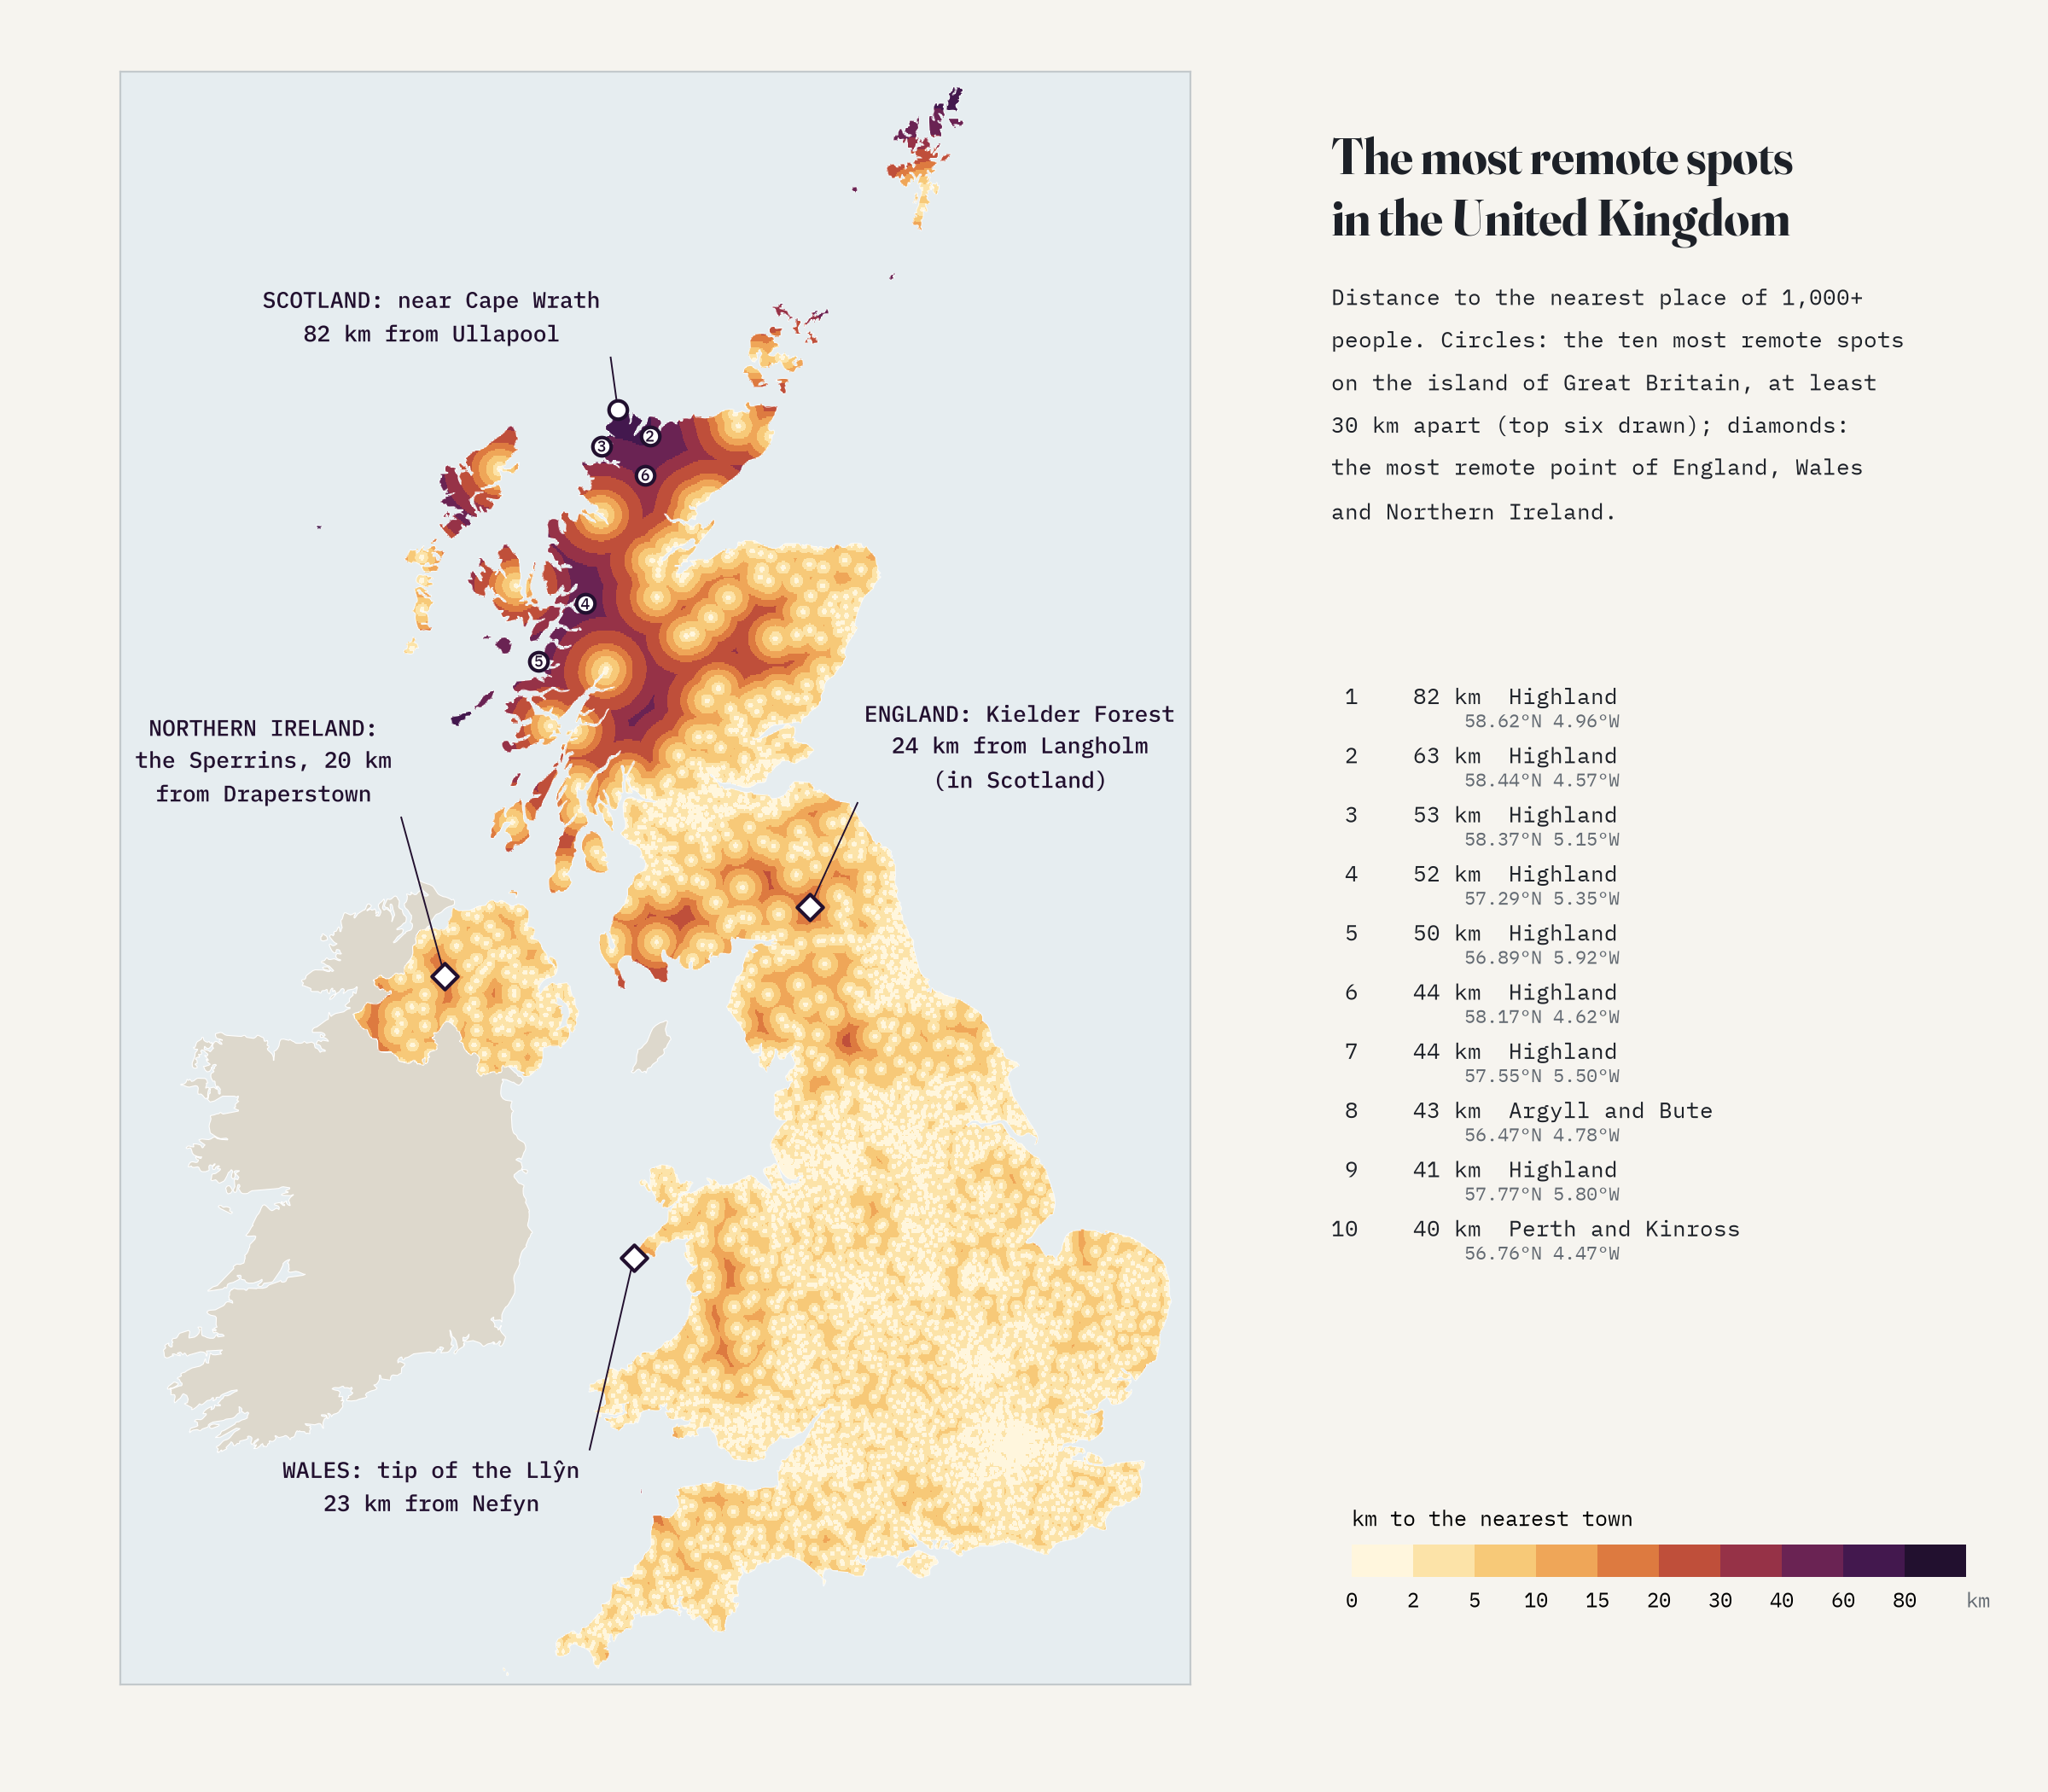
\includegraphics[width=0.9\textwidth]{f_uk.png}
\caption{Distance to the nearest place of 1,000 or more people in the United Kingdom, computed on a 0.01 degree grid, with the most remote point of each nation and the ten most remote spots on Great Britain.}\label{fig:uk}\end{figure}

\section{Limitations}
First, the gazetteer threshold matters. Cities1000 omits villages and hamlets under 1,000 people, so a point far from a town may still be close to people: Inuit hamlets in the Canadian Arctic, Saharan oases, cattle stations in Australia and research stations in Antarctica. It also keeps a few smaller administrative seats, such as Port-aux-Fran\c{c}ais on Kerguelen and Grytviken on South Georgia, which shortens some island distances. Second, populations in Natural Earth are estimates of differing dates. Third, straight-line distance is not travel time: terrain, water, roads and borders all intervene. The Malaria Atlas Project's global accessibility map for 2015 \citep{weiss2018} measures travel time to cities and is a complementary view. Fourth, the 0.1 degree grid and the 1:50m coastline smooth small islands and narrow inlets; the maxima are refined to about a kilometre, but the shares are grid estimates. Fifth, continents and mainlands are conventions, and the Europe and Asia split in Russia is approximate.

\section{Conclusion}
Measured from people rather than from the sea, the most remote places on Earth are not where the classic poles of inaccessibility lie. They are on the ice and islands of the high latitudes and the Southern Ocean, and on the mainlands in the high Arctic, the Australian and Saharan deserts and the far north of Canada. A quarter of the land outside Antarctica is more than 100 km from a town of 1,000 people, but only about one per cent is more than 500 km away, and in a country like Britain the middle of nowhere is never more than 82 km from a town.

\section*{Data and code availability}
The interactive map is at \url{https://maps.tristanhotham.com/remote-places/}. Data and code are at \url{https://github.com/Tristan-Hotham/remote-places} and archived with this paper at https://doi.org/10.5281/zenodo.23873015. Derived data are released under CC BY 4.0 and code under the MIT licence. Town data: GeoNames, CC BY 4.0. Natural Earth is public domain.

\section*{AI statement}
I wrote the text, with drafting and editing assistance from Claude (Anthropic), which also helped prepare the analysis code. I reviewed and checked all text and results.

\begin{thebibliography}{9}
\bibitem[GeoNames(2026)]{geonames} GeoNames (2026) cities1000: all cities with a population of 1,000 or more. CC BY 4.0. \url{https://www.geonames.org/}
\bibitem[lutangar(2026)]{citiesjson} lutangar (2026) cities.json: GeoNames cities1000 as JSON, commit e5e759c56751bd7329e29c576f6a9e77607b424e. \url{https://github.com/lutangar/cities.json}
\bibitem[Natural Earth(2026)]{naturalearth} Natural Earth (2026) Populated places, land, admin 0 countries and admin 1 states and provinces, 1:50m and 1:10m. Public domain. \url{https://www.naturalearthdata.com/}
\bibitem[Weiss et al.(2018)]{weiss2018} Weiss, D. J. and others (2018) A global map of travel time to cities to assess inequalities in accessibility in 2015. \textit{Nature}. Malaria Atlas Project, University of Oxford.
\end{thebibliography}
\end{document}
